\documentclass{article}
\usepackage{tikz}
\usetikzlibrary{calc}

\begin{document}

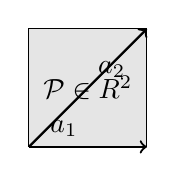
\begin{tikzpicture}[scale=1.5]
    % Define the vertices of the parallelogram in R^2
    \coordinate (A) at (0,0);
    \coordinate (B) at (1,0);
    \coordinate (C) at (1,1);
    \coordinate (D) at (0,1);

    % Draw the parallelogram
    \draw[fill=gray!20] (A) -- (B) -- (C) -- (D) -- cycle;

    % Draw the vectors
    \draw[->, thick] (A) -- node[above left] {$a_1$} (B);
    \draw[->, thick] (A) -- node[above right] {$a_2$} (C);

    % Label the point P
    \node at (0.5,0.5) {$\mathcal{P} \in \mathbb{R}^2$};
\end{tikzpicture}

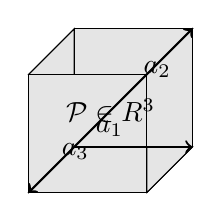
\begin{tikzpicture}[scale=1.5]
    % Define the vertices of the parallelepiped in R^3
    \coordinate (A) at (0,0,0);
    \coordinate (B) at (1,0,0);
    \coordinate (C) at (1,1,0);
    \coordinate (D) at (0,1,0);
    \coordinate (E) at (0,0,1);
    \coordinate (F) at (1,0,1);
    \coordinate (G) at (1,1,1);
    \coordinate (H) at (0,1,1);

    % Draw the parallelepiped
    \draw[fill=gray!20] (A) -- (B) -- (F) -- (E) -- cycle;
    \draw[fill=gray!20] (B) -- (C) -- (G) -- (F) -- cycle;
    \draw[fill=gray!20] (C) -- (D) -- (H) -- (G) -- cycle;
    \draw[fill=gray!20] (D) -- (A) -- (E) -- (H) -- cycle;
    \draw[fill=gray!20] (A) -- (B) -- (C) -- (D) -- cycle;
    \draw[fill=gray!20] (E) -- (F) -- (G) -- (H) -- cycle;

    % Draw the vectors
    \draw[->, thick] (A) -- node[above left] {$a_1$} (B);
    \draw[->, thick] (A) -- node[above right] {$a_2$} (C);
    \draw[->, thick] (A) -- node[above right] {$a_3$} (E);

    % Label the point P
    \node at (0.5,0.5,0.5) {$\mathcal{P} \in \mathbb{R}^3$};
\end{tikzpicture}

\end{document}